\documentclass[main.tex]{subfiles}

\begin{document}
The central value is not set in stone yet.
However, most of the systmatic effects can still be calculated.
The effect with the lower beta cut is likely due to the normalization of the beta-gamma sum spectrum.
The issue is a solvable oen. 

\section{Discussion of Results}

The statistical uncertainty of the lower beta cut effect is 0.0042.
This is with 7 million events that pass the filter.
If the lower beta cut uncertainty is excluded, the total systematic uncertainty is 0.0036.
This also excludes any uncertainty on the offset in the calibration and the normalization of the gamma-beta sum spectrum.
This is dominated by the uncertainty on the weak magnetism.
If the lower beta cut uncertainty can be resolved, the total systematic uncertainty should only be a touch higher than 0.0036.
This is very close to the statistical uncertainty. 

To lower the systematic uncertainty, the weak magnetism should be known to a more percsise value.
The uncertainty of the weak magnetism comes from how it is calcualted.
The parameters need to cacluated the weak magnestism are shown in equation \ref{eq:bwmcal} .
Most of the uncertainty comes from the gamma decay strength \cite{Min11}.
A better measurement of this gamma decay strength would reduce the effect of the weak magnetism.

\section{Results Compared to Other Measurements of the Fierz Term}

A similar measurement was done with ultra-cold neutrons \cite{Hic17}.
The beta decay spectrum was measured using a magnetic spectrometer.
The neutrons were confined in the cter with a magnetic field, and allowed to decay.
A superratio was used to extract the Fierz term.
With the systematic effects, the final results of the Fierz term was $0.067 \pm 0.005_{stat} ^{+0.090}_{-0.061 sys}$.
Even with the lower beta cut effect, the systematic uncertainty of the Fierz term in the $^{20}$F measurement is much smaller.
The statistical uncertainty is comparable. 
Additionally, since the decay of a neutron is a mixed decay, this Fierz term is sensitive to both the tensor couplings and the scalar couplings.  
The beta spectrum is shown in figure \ref{fig:ucnabeta}.

\begin{figure}[!htb]
	\centerline{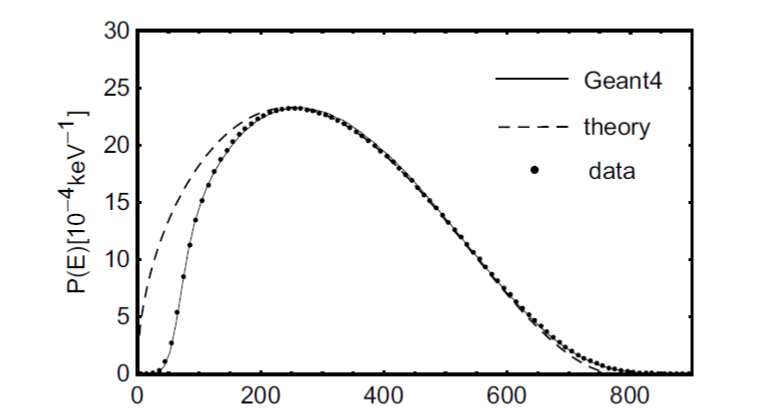
\includegraphics[width=0.78\textwidth]{NeutronBetaSpectrumUCNA.png}}
	\caption{The energy spectrum of the ultra-cold neutron measurement \cite{Hic17}}
	\label{fig:ucnabeta}
\end{figure}

There are large distortions at low energy due to back-scattering effects. 
The systematic uncertainty quoted due to backscattering effects is $\pm 0.005$, which is larger the statistical uncertianty of this $^{20}$F measurement.
The largest systematic uncertainty in the neutron measurement was due to uncertainties in the detector calibration.
The fluorine measurement avoids this, as the gain is left as a free parameter.

Another method to get the Fierz term is by measuring $ft$ values.
From the superallowed beta decays, the result for the Fierz term is $-0.0028 \pm 0.0026$ \cite{Har17}.
It was obtained with $ft$ vaule measurements of 14 different nuclei. 
The uncertainty is the statistical uncertainty of the fit after the $ft$ values were corrected.
However, this Fierz term is sensitive to scalar couplings, and not tensor coupling like in the $^{20}$F measurement.
It had different systematic effects, and it took 14 different measurements to come up with this number.
Even with all this, the potential sensitivity to the implant technique is similar to that of 14 $ft$ value measurements.

A different measurement with sensitivty to tensor couplings was made with $^{60}$Co \cite{Wau10}.
This measurement measured the beta assymetry.
Then, this asymetry was compared to the standard model value.
This was done with a large magnet. 
The largest uncertainty was due to the size and location of the source.
The limit on the tensor couplings was between $-0.089$ and $0.013$.
Assuming that $C_{A}' = 0$, this corresponds to a simular error bar in the Fierz term.
This uncertainty is larger than the uncertainty due to the lower beta cut effect.

\section{Further Refinements to Technique}
\end{document}
